Одним из простых опытов, подтверждающих существование дискретных уровней энергии
атомов, является эксперимент, известный под названием опыта Франка и Герца.
Схема опыта изображена на рис. \ref{pic1}.

\begin{figure}[h]
  \center
  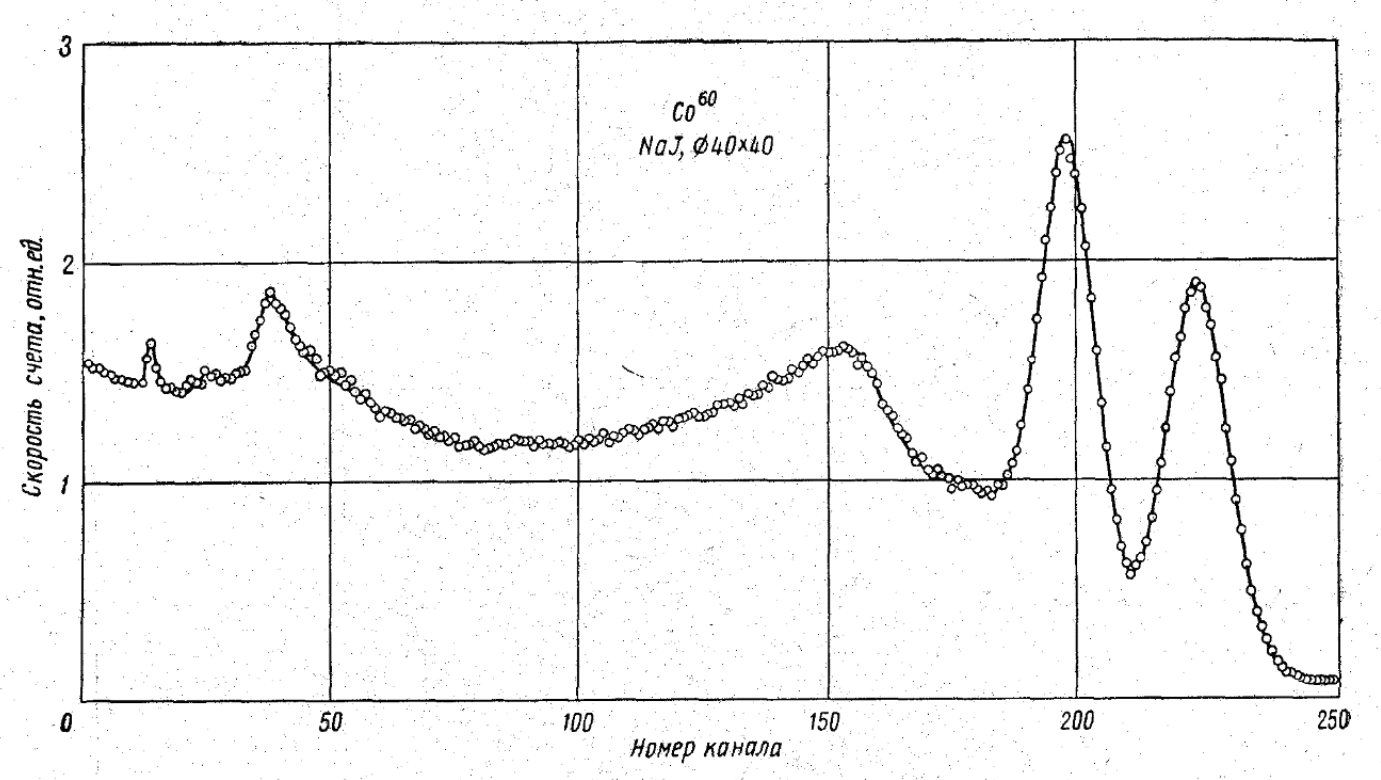
\includegraphics[width=0.8\linewidth]{pic1.png}
  \caption{ Принципиальная схема опыта Франка и Герца }
  \label{pic1}
\end{figure}

Разреженный одноатомный газ ( в нашем случае -- гелий ) заполняет
трёхэлектродную лампу. Электроны, испускаемые разогретым катодом, ускоряются в
постоянном электрическом поле, созданным между катодом и сетчатым анодом лампы.
Передвигаясь от катода к аноду, электроны сталкиваются с атомами гелия. Если
энергия электрона, налетающего на атом, недостаточна для того, чтобы перевести
его в возбуждённое состояние ( или ионизовать ), то возможны только упругие
соударения, при которых электроны почти не теряют энергии, так как их масса в
тысячи раз меньше массы атомов.

По мере увеличения разности потенциалов между анодом и катодом энергия
электронов увеличивается и, в конце концов, оказывается достаточной для
возбуждения атомов. При таких -- неупругих -- столкновениях кинетическая энергия
налетающего электрона передаётся одному их атомных электронов, вызывая его
переход на свободный энергетический уровень (возбуждение) или совсем отрывая его
от атома (ионизация)

Третьим электродом лампы является коллектор. Между ним и анодом поддерживается
небольшое задерживающее напряжение (потенциал коллектора меньше потенциала
анода)ю Ток коллектора, пропорциональный числу попадающих на него за секунду
электронов, изменяется микроамперметром.

\begin{figure}[h]
  \center
  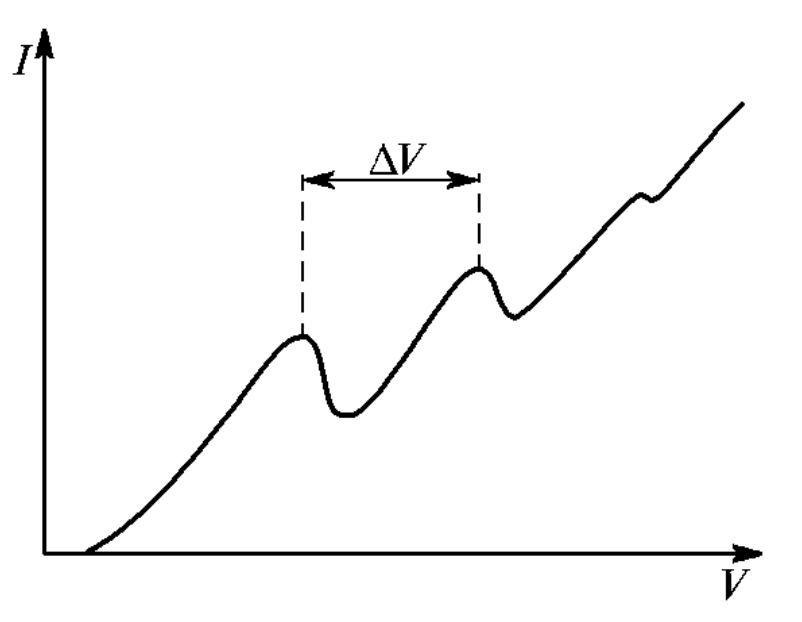
\includegraphics[width=0.7\linewidth]{pic2.png}
  \caption{ Зависимость тока коллектора от напряжения на аноде }
  \label{pic2}
\end{figure}

При увеличении потенциала анода ток в лампе вначале растёт, подобно тому как это
происходит в вакуумном диоде (рис. \ref{pic2}). Однако, когда энергия электронов
становится достаточной для возбуждения атомов, ток коллектора резко уменьшается.
Это происходит потому, что пр неупругих соударениях с атомами электроны почти
полностью теряют свою энергию и не могут преодолеть задерживающего потенциала
(около $1$В) между анодом и коллектором. При дальнейшем движении к аноду
успевают набрать энергию, достаточную для преодоления задерживающего потенциала.

Следующее замедление роста тока происходит в момент, когда часть электронов
неупруго сталкивается с атомами два раза: первый раз посередине пути, второй --
у анода, и т.д. Таким образом, на кривой зависимости тока коллектора от
напряжения анода имеется ряд максимумов и минимумов, отстоящих друг от друга на
равные расстояния $\Delta V$; эти расстояния равны энергии первого возбуждённого
состояния (рис. \ref{pic2}).

При тщательной постановке опыта можно увидеть и тонкую структуру кривой спада
тока, содержащую ряд минимумов, соответствующих возбуждению других уровней и
ионизации атома гелия. Для этого нужны лампы специальной конструкции. В нашей
постановке опыта эта тонкая структура не видна.